% !TeX program = xelatex
% Encoding: UTF-8. Compile twice with XeLaTeX or use latexmk -xelatex.
% Content snapshot: 03/10/2026; LaTeX conversion: 04/10/2026.
% Edit report metadata below. All figures use relative paths.
\documentclass[12pt,letterpaper]{article}
\usepackage{fontspec}
\IfFontExistsTF{Times New Roman}{\setmainfont{Times New Roman}}{\setmainfont{TeX Gyre Termes}}
\IfFontExistsTF{Arial}{\setsansfont{Arial}}{\setsansfont{TeX Gyre Heros}}
\IfFontExistsTF{Consolas}{\setmonofont{Consolas}[Scale=0.85]}{\setmonofont{Latin Modern Mono}[Scale=0.85]}
\usepackage[vietnamese]{babel}
\usepackage[left=3cm,right=2cm,top=2cm,bottom=2cm]{geometry}
\usepackage{amsmath,amssymb}
\usepackage{graphicx}
\usepackage[table]{xcolor}
\usepackage{array,float}
\usepackage{caption}
\usepackage{enumitem}
\usepackage{setspace}
\usepackage{titlesec}
\usepackage{tocloft}
\usepackage{xurl}
\usepackage[unicode,hidelinks]{hyperref}

\definecolor{tablehead}{HTML}{333333}
\definecolor{tableborder}{HTML}{D9D9D9}
\definecolor{tablerow}{HTML}{F4F4F4}
\newlength{\tablebodywidth}
\setstretch{1.12}
\setlength{\parindent}{0pt}
\setlength{\parskip}{5pt}
\setlength{\intextsep}{8pt}
\setlength{\emergencystretch}{2em}
\setcounter{tocdepth}{1}
\setcounter{secnumdepth}{1}
\setlist[enumerate]{leftmargin=*,itemsep=3pt,topsep=4pt,parsep=0pt}
\titleformat{\section}{\color{black}\bfseries\fontsize{15.5}{18}\selectfont}{\thesection}{0.6em}{}
\titleformat{\subsection}{\color{black}\bfseries\fontsize{13}{15}\selectfont}{}{0pt}{}
\titlespacing*{\section}{0pt}{0pt}{8pt}
\titlespacing*{\subsection}{0pt}{7pt}{4pt}
\captionsetup{font=small,labelfont=bf,labelsep=space,justification=raggedright,singlelinecheck=false,skip=5pt}
\captionsetup[table]{position=top}
\renewcommand{\contentsname}{Mục lục}
\renewcommand{\tablename}{Bảng}
\renewcommand{\figurename}{Hình}
\renewcommand{\cftsecfont}{\normalfont}
\renewcommand{\cftsecpagefont}{\normalfont}
\renewcommand{\cftsecleader}{\cftdotfill{\cftdotsep}}
\setlength{\cftbeforesecskip}{4pt}
\setlength{\cftsecnumwidth}{1.5em}
\setlength{\cftbeforetoctitleskip}{0pt}
\setlength{\cftaftertoctitleskip}{8pt}
\hypersetup{pdftitle={Báo cáo tiến độ kỹ thuật hệ thống MPU6050 và ADS1292R},pdfauthor={Trần Đức Trí; Trần Nguyễn Phúc Bình; Nguyễn Phú Minh}}

\begin{document}
% ------------------------------------------------------------
% Cover page
% ------------------------------------------------------------
\begin{titlepage}
\centering
{\fontsize{14}{18}\selectfont TRƯỜNG ĐẠI HỌC BÁCH KHOA HÀ NỘI\par}
\vspace{0.6cm}
{\fontsize{14}{18}\selectfont THIẾT BỊ ĐEO THEO DÕI TIẾN TRÌNH MỎI CƠ\par}
\vspace{0.9cm}
{\fontsize{24}{29}\selectfont\bfseries Báo cáo tiến độ kỹ thuật hệ thống MPU6050 và ADS1292R\par}
\vspace{0.7cm}
{\fontsize{14}{18}\selectfont Thiết bị đeo theo dõi chuyển động và tín hiệu điện cơ trong bài tập kháng lực\par}
\vspace{0.5cm}
{\fontsize{14}{18}\selectfont Báo cáo tiến độ kỹ thuật\par}
\vspace{0.5cm}
Nhóm thực hiện\par
Trần Đức Trí\par
Trần Nguyễn Phúc Bình\par
Nguyễn Phú Minh\par
\vspace{0.6cm}
Ngày 03 tháng 10 năm 2026\par
Hà Nội năm 2026\par
\thispagestyle{plain}
\end{titlepage}
\setcounter{page}{2}


% ------------------------------------------------------------

% Mục lục và tóm tắt tiến độ

% ------------------------------------------------------------

\tableofcontents

\vspace{5pt}

\subsection*{Tóm tắt tiến độ}

Nhóm đã phát triển hai luồng firmware trên ESP32 S3. Nhánh MPU6050 thu gia tốc, vận tốc góc, nhiệt độ và dấu nút bấm; các công cụ Python lưu CSV và tạo biểu đồ. Nhánh ADS1292R thu hai kênh ADC 24 bit theo ngắt, xử lý kênh 2 bằng bộ lọc số, ghi CSV và hiển thị trực tiếp trên trình duyệt.


Kết quả hiện có là nền tảng thu và quan sát dữ liệu. Hai cảm biến chưa được thu đồng thời trong một firmware; chưa có thuật toán velocity loss hoặc mô hình FCF (tỉ lệ số rep đã hoàn thành trong set đến failure) và RIR (số rep còn lại đến failure) chạy trên ESP32. Hiệu quả lọc nhiễu ADS cần được xác nhận bằng phép đo trước và sau lọc.


Ưu tiên tiếp theo là kiểm tra thang đo MPU, thu dữ liệu ADS liên tục, xác định pha nâng của từng rep và xây dựng phép đo tham chiếu. Các kết quả build và kiểm thử phần mềm được trình bày riêng với các phép đo phần cứng chưa thực hiện.


% ------------------------------------------------------------

% 1 Tổng quan hệ thống và phạm vi triển khai

% ------------------------------------------------------------

\clearpage

\section{Tổng quan hệ thống và phạm vi triển khai}

Hệ thống hướng tới theo dõi tiến trình mỏi cơ trong bài tập kháng lực bằng thông tin chuyển động và hoạt động điện cơ bề mặt. MPU6050 hỗ trợ quan sát động tác, xác định chu kỳ lặp và khảo sát sự giảm tốc độ. ADS1292R cung cấp tín hiệu điện thế sinh học để nghiên cứu biên độ và phổ sEMG. Mỗi loại dữ liệu cần cách thu, lọc và kiểm chứng riêng.


\begin{table}[H]
\centering
\caption{So sánh hai luồng đang triển khai}
\begingroup
\fontsize{10.5}{12.5}\selectfont
\setlength{\tabcolsep}{5pt}
\setlength{\tablebodywidth}{\dimexpr\linewidth-6\tabcolsep-4\arrayrulewidth\relax}
\renewcommand{\arraystretch}{1.2}
\arrayrulecolor{tableborder}
\begin{tabular}{|>{\raggedright\arraybackslash}p{0.188889\tablebodywidth}|>{\raggedright\arraybackslash}p{0.405556\tablebodywidth}|>{\raggedright\arraybackslash}p{0.405556\tablebodywidth}|}
\hline
\rowcolor{tablehead}
{\color{white}\bfseries Hạng mục} & {\color{white}\bfseries MPU6050} & {\color{white}\bfseries ADS1292R} \\ \hline
Nhánh được đối chiếu & dev-mpu tại d2aaa81 & binhdev-ads tại 3a67a0a \\ \hline
\rowcolor{tablerow}
Giao tiếp cảm biến & I\textsuperscript{2}C 100 kHz & SPI 1 MHz và MODE1 \\ \hline
Nhịp đọc mục tiêu & 100 mẫu mỗi giây & 2000 mẫu mỗi giây \\ \hline
\rowcolor{tablerow}
Dữ liệu chính & Gia tốc và gyro ba trục, nhiệt độ, button & Raw hai kênh 24 bit, filtered kênh 2, sequence và timestamp \\ \hline
Công cụ quan sát & PNG và dashboard HTML từ file CSV & Web trực tiếp và recorder CSV \\ \hline
\end{tabular}
\endgroup
\end{table}

\subsection*{Luồng dữ liệu và lý do tổ chức}

Với MPU, ESP32 đọc cảm biến theo lịch 10 ms và gửi từng dòng CSV; máy tính lưu dữ liệu rồi tạo biểu đồ. Cách tổ chức này phục vụ khảo sát chuyển động và đối chiếu dấu nút bấm. Dashboard IMU hiển thị bản ghi đã lưu, chưa phải công cụ nhận Serial trực tiếp.


Với ADS, cạnh DRDY báo có mẫu mới. Tác vụ thu đọc SPI, đẩy mẫu vào hàng đợi, sau đó main xử lý DSP và gửi Serial. Máy tính tiếp nhận dữ liệu mẫu đầy đủ để ghi CSV; một luồng trạng thái có nhịp thấp hơn phục vụ giao diện. Việc tách hai luồng giảm tải hiển thị mà vẫn giữ dữ liệu nhận được để phân tích.


\subsection*{Trạng thái chức năng}

Firmware hiện chưa kết hợp MPU và ADS trong cùng một chương trình. Các bước đếm rep, đồng bộ hai cảm biến, velocity loss, trích xuất đủ bộ đặc trưng nghiên cứu và suy luận mô hình trên chip còn cần triển khai. Công cụ \path{analyze_semg.py} từng có trong phiên bản trước đã được xóa khỏi thư mục làm việc hiện tại; các kết quả khảo sát offline trước đây chưa được xem là chức năng đang hoạt động.


% ------------------------------------------------------------

% 2 Thu dữ liệu MPU6050 và bộ lọc tích hợp

% ------------------------------------------------------------

\clearpage

\section{Thu dữ liệu MPU6050 và bộ lọc tích hợp}

Firmware MPU sử dụng Wire để ghi cấu hình và đọc trực tiếp thanh ghi cảm biến. Một lần đọc lấy 14 byte chứa gia tốc ba trục, nhiệt độ và vận tốc góc ba trục. Dữ liệu nguyên có dấu được quy đổi sang đơn vị vật lý trước khi xuất CSV. Nút bấm bổ sung mốc thao tác thủ công để đối chiếu với dạng sóng.


\begin{table}[H]
\centering
\caption{Cấu hình MPU trong nhánh dev mpu}
\begingroup
\fontsize{10.5}{12.5}\selectfont
\setlength{\tabcolsep}{5pt}
\setlength{\tablebodywidth}{\dimexpr\linewidth-6\tabcolsep-4\arrayrulewidth\relax}
\renewcommand{\arraystretch}{1.2}
\arrayrulecolor{tableborder}
\begin{tabular}{|>{\raggedright\arraybackslash}p{0.305556\tablebodywidth}|>{\raggedright\arraybackslash}p{0.261111\tablebodywidth}|>{\raggedright\arraybackslash}p{0.433333\tablebodywidth}|}
\hline
\rowcolor{tablehead}
{\color{white}\bfseries Thông số} & {\color{white}\bfseries Giá trị} & {\color{white}\bfseries Ý nghĩa} \\ \hline
SDA và SCL & GPIO 18 và 17 & Giao tiếp I\textsuperscript{2}C với địa chỉ 0x68 \\ \hline
\rowcolor{tablerow}
Gia tốc & \ensuremath{\pm}4 g và 8192 LSB mỗi g & Quy đổi raw thành gia tốc theo g \\ \hline
Gyro & \ensuremath{\pm}500 \ensuremath{^{\circ}}/s và 65,5 LSB mỗi \ensuremath{^{\circ}}/s & Quy đổi raw thành vận tốc góc \\ \hline
\rowcolor{tablerow}
Bộ lọc \path{DLPF_CFG} & 3 qua CONFIG bằng 0x03 & Accel 44 Hz và gyro 42 Hz \\ \hline
Nhịp đọc của ESP32 & 100 Hz và chu kỳ 10 ms & Lịch lấy dữ liệu gửi lên máy tính \\ \hline
\rowcolor{tablerow}
Serial và button & 921600 baud và GPIO 5 & Nhấn nút được mã hóa bằng 1 \\ \hline
\end{tabular}
\endgroup
\end{table}

\subsection*{Tại sao dùng thông thấp 44 Hz}

DLPF là bộ lọc số tích hợp trong MPU. Cấu hình đang dùng giảm dao động nhanh và nhiễu cảm biến, giúp quan sát chuyển động rõ hơn. Datasheet quy định băng thông accel 44 Hz với độ trễ 4,9 ms và gyro 42 Hz với độ trễ 4,8 ms ở cấu hình 3. Vì vậy, ghi chú chung 44 Hz trong code cần được hiểu chính xác cho từng loại tín hiệu \hyperlink{ref1}{[1]}.


ESP đọc ở 100 Hz nên giới hạn Nyquist của chuỗi dữ liệu là 50 Hz. Băng thông 44 và 42 Hz nằm dưới giới hạn đó nhưng bộ lọc không cắt đứt phổ tại tần số này. Cấu hình chưa bảo đảm triệt hoàn toàn aliasing. \path{SMPLRT_DIV} bằng 0 tạo cập nhật nội bộ 1 kHz khi DLPF bật, trong khi ESP chỉ đọc mỗi 10 ms \hyperlink{ref1}{[1]}.


\subsection*{Các giới hạn cần xử lý}

main chưa có FIFO, sequence hoặc thống kê mất mẫu cho MPU. Timestamp millis được lấy sau khi đọc; các khoảng cách timestamp đều chưa chứng minh thời điểm đọc không có jitter. Firmware cũng chưa hiệu chuẩn bias gyro, loại trọng lực, xác định góc hay dùng \path{KalmanFilter.h.} Với velocity loss, cần đánh giá ảnh hưởng của bộ lọc lên thời gian pha nâng và vận tốc từng rep trước khi chọn cấu hình cuối cùng.


% ------------------------------------------------------------

% 3 Dữ liệu MPU và kết quả quan sát

% ------------------------------------------------------------

\clearpage

\section{Dữ liệu MPU và kết quả quan sát}

Bản ghi có sẵn trong nhánh dev-mpu gồm 6066 dòng, kéo dài 60,65 giây. Có 6065 khoảng cách timestamp đều bằng 10 ms và 264 dòng mang button bằng 1. Đây là dữ liệu lưu trong repo, dùng minh họa chức năng ghi và trực quan hóa; các con số này không được gán cho hai ảnh dashboard mới đã trao đổi.


\begin{figure}[H]
\centering
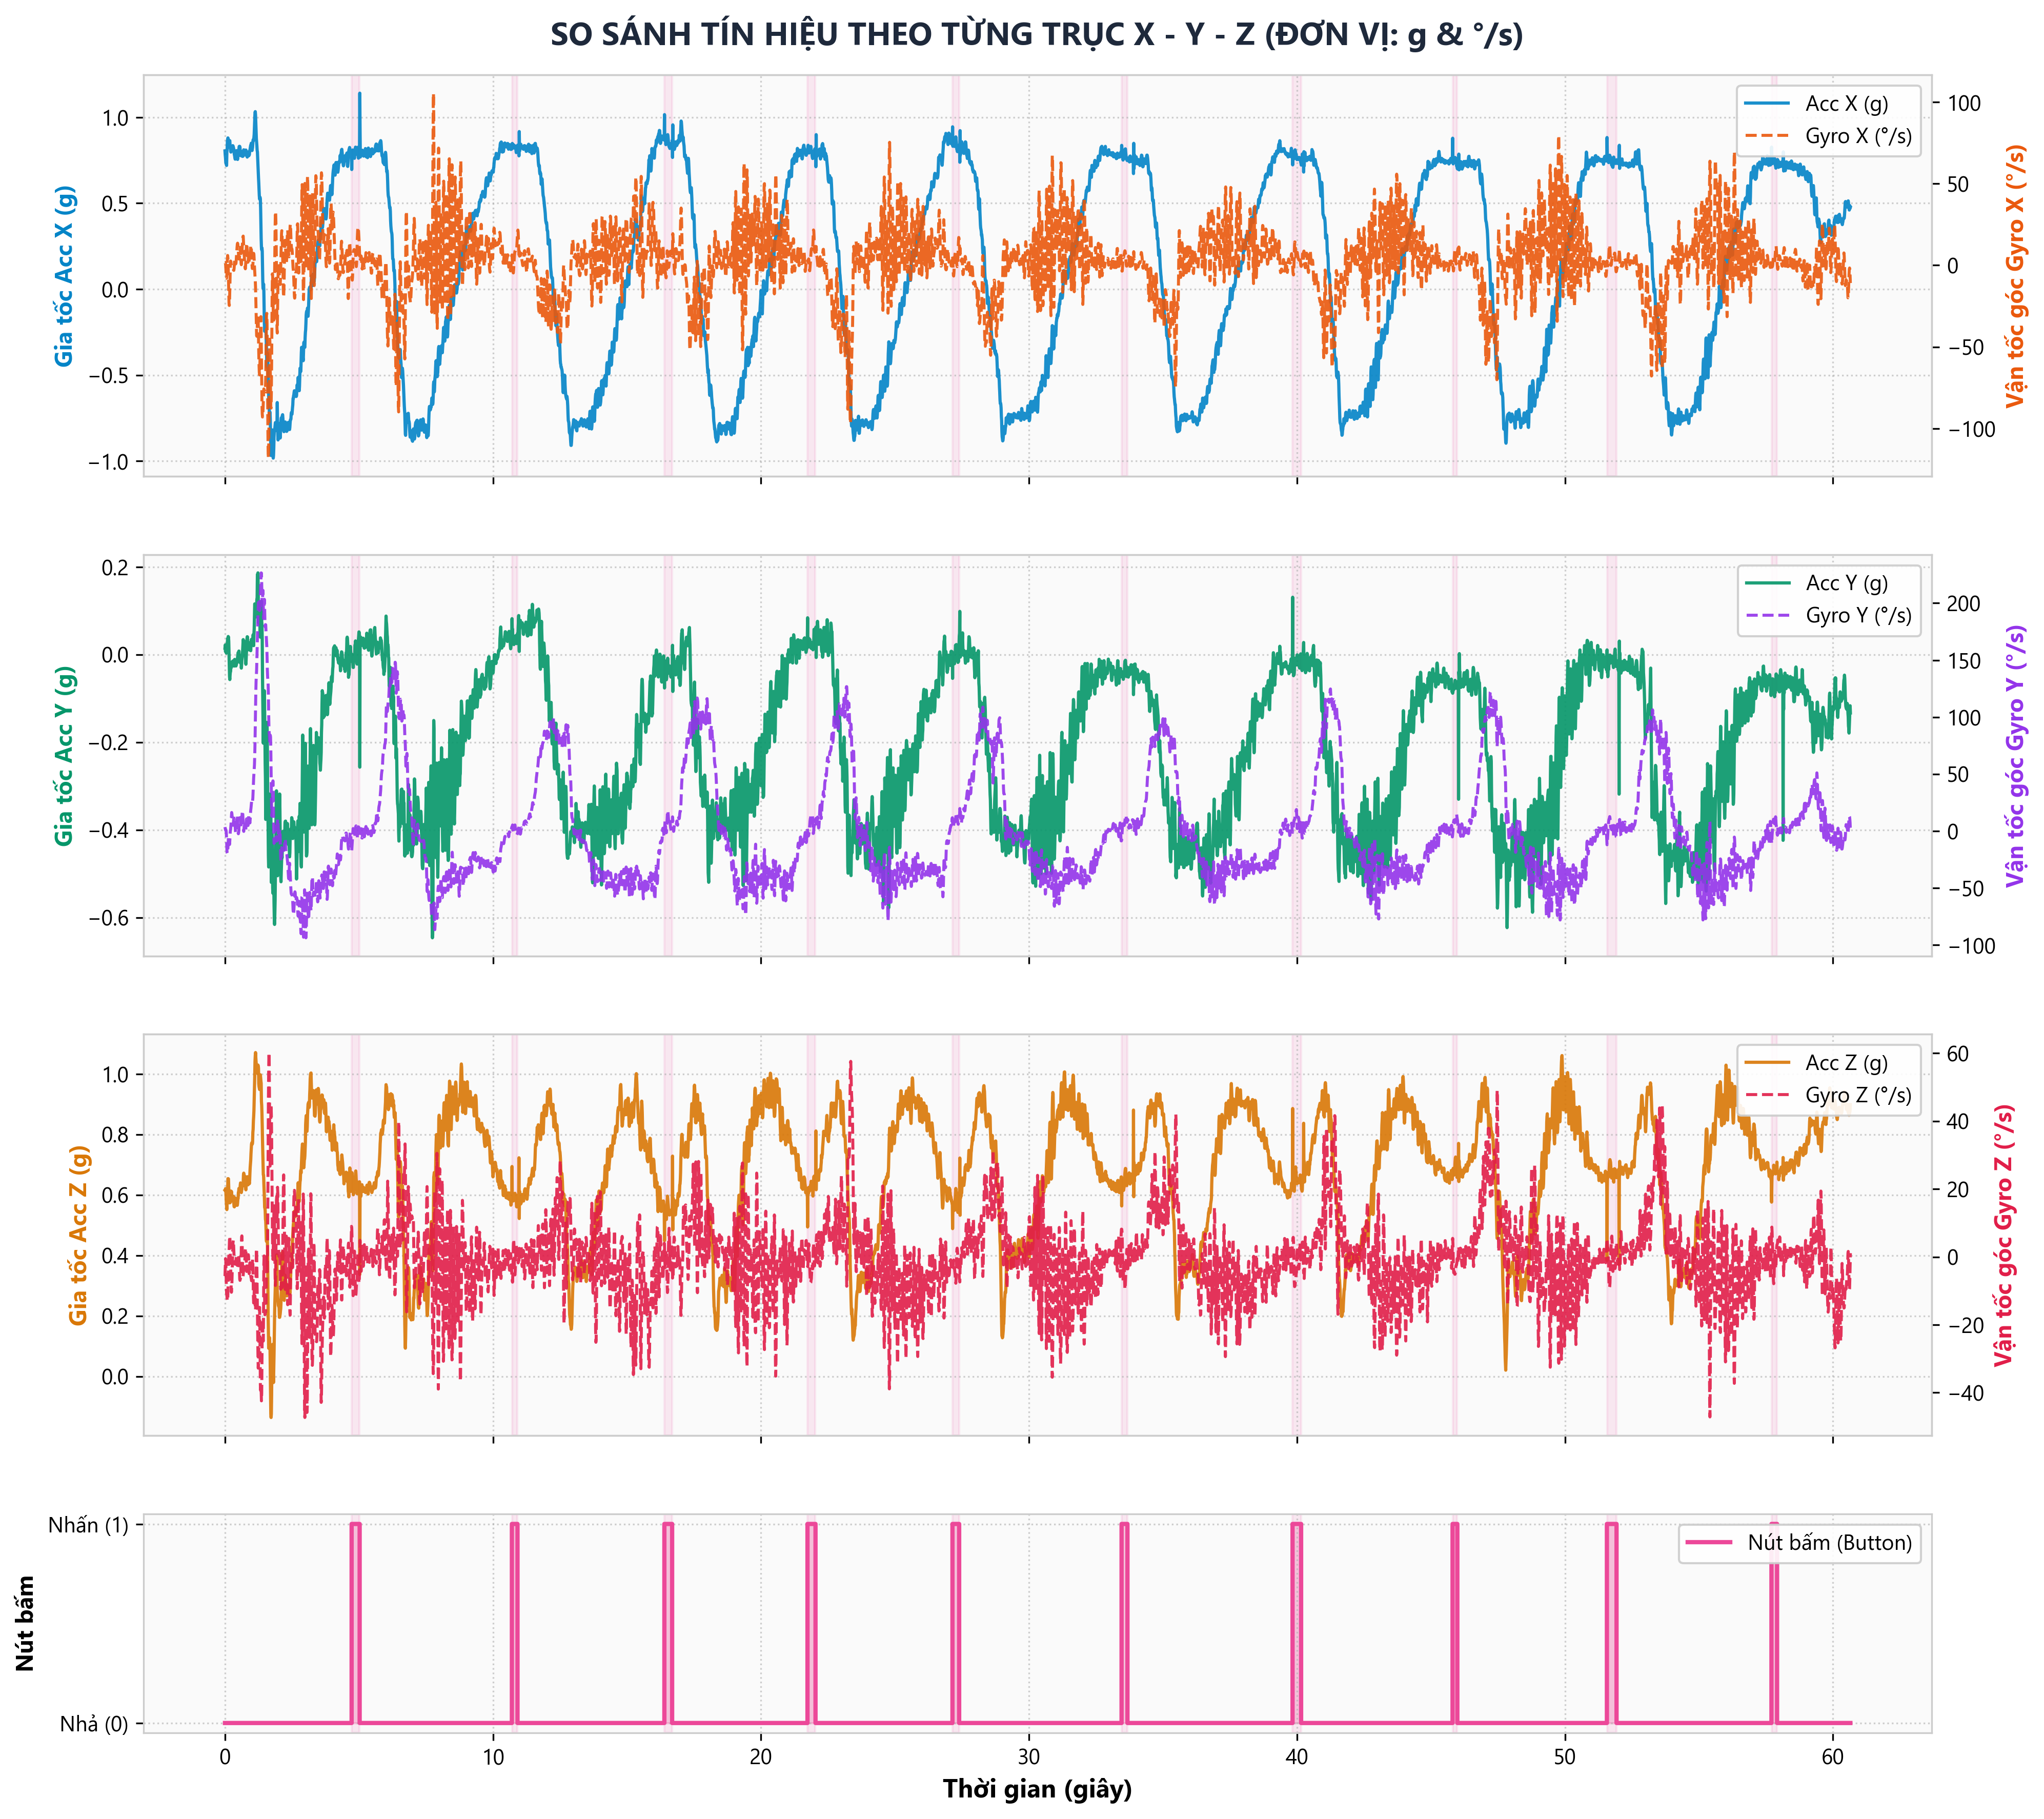
\includegraphics[width=0.86\linewidth]{assets/mpu-plot_axes_xyz_breakdown.png}
\caption{Gia tốc và gyro theo từng trục cùng dấu nút bấm trong bản ghi MPU của nhánh dev mpu}
\label{fig:mpu-data}
\end{figure}

Các công cụ đã tạo bốn hình PNG và dashboard Plotly để xem từng trục, độ lớn vector, phân bố, tương quan và phổ. Dạng sóng lặp lại là cơ sở khảo sát tách rep. Đồ thị 3D hiện biểu diễn vector gia tốc, chưa phải quỹ đạo vị trí của cảm biến.


Trong hai ảnh dashboard mới, chu kỳ chuyển động xuất hiện khá rõ, đồng thời có xung đầu bản ghi và các dao động nhanh. Độ lớn gia tốc nhìn gần 2 g cần kiểm tra bằng dữ liệu tĩnh. Nếu cảm biến đứng yên mà giá trị vẫn gần 2 g, phải đối chiếu \path{ACCEL_CONFIG} và hệ số quy đổi trước khi tính vận tốc. Những nhận xét từ ảnh chưa đủ xác nhận nhiễu, số rep hoặc mức mỏi.


% ------------------------------------------------------------

% 4 Hướng đánh giá velocity loss bằng MPU

% ------------------------------------------------------------

\clearpage

\section{Hướng đánh giá velocity loss bằng MPU}

Velocity loss biểu diễn mức giảm vận tốc của một rep so với vận tốc tham chiếu trong set. Rep là một lần lặp động tác; set là một hiệp gồm nhiều rep. Nghiên cứu trên tập kháng lực đã ghi nhận quan hệ giữa sự giảm vận tốc và các chỉ báo mỏi thần kinh cơ \hyperlink{ref4}{[4]}. Trong project, đây là hướng sử dụng dữ liệu MPU để theo dõi suy giảm hiệu suất, đồng thời kiểm chéo kết quả từ sEMG.


\[\mathrm{VL}_k=\frac{v_{\mathrm{ref}}-v_k}{v_{\mathrm{ref}}}\times100\%\]

\(v_{\mathrm{ref}}\) là vận tốc tham chiếu được định nghĩa trước; \(v_k\) là vận tốc rep k, được tính theo cùng đại lượng và cùng pha chuyển động. Ví dụ, vận tốc trung bình pha nâng giảm từ 0,60 \path{m/s} xuống 0,45 \path{m/s} thì VL bằng 25\%. Giá trị này mô tả mức giảm vận tốc; nó chưa trực tiếp xác định FCF, RIR hoặc phần trăm mỏi cơ.


\subsection*{Chọn đại lượng từ gyro}

Gyro đo vận tốc góc, đơn vị \ensuremath{^{\circ}}/s. Với động tác có trục quay rõ và cảm biến gắn chắc, có thể khảo sát vận tốc góc trung bình trong pha nâng sau khi trừ bias. Cần chọn trục hoặc phép chiếu lên trục chuyển động đã xác định. Độ lớn vector gyro gộp ba trục và mất dấu chiều quay, nên một đỉnh của đường này chưa đủ xác định một rep.


Khi dùng vận tốc góc, báo cáo kết quả dưới tên mức giảm vận tốc góc và kiểm chứng khả năng đại diện cho động tác. Quan hệ v bằng r nhân omega chỉ áp dụng cho mô hình quay với bán kính đã biết; không thể tự áp dụng cho mọi vị trí gắn MPU. Muốn suy ra vận tốc tuyến tính từ accel, cần xác định hướng, loại trọng lực và kiểm soát trôi tích phân.


\subsection*{Các bước triển khai đề xuất}

\begin{enumerate}

\item Hiệu chuẩn thang đo và bias, gắn cảm biến chắc, ghi video tham chiếu cùng bản ghi.

\item Tách từng rep, xác định pha nâng và kiểm tra biên độ chuyển động của pha đó.

\item Tính vận tốc trung bình pha nâng và chọn tham chiếu từ các rep đầu hợp lệ theo quy tắc đã khai báo.

\item Tính VL từng rep, giữ tải và kỹ thuật tương đối nhất quán, ghi nhận nhịp chủ động của người tập.

\item Đối chiếu số rep, ranh giới pha và sai số vận tốc với video hoặc thiết bị tham chiếu trước khi kết luận về mỏi.

\end{enumerate}

Cần báo cáo riêng sai số đo và mức giảm quan sát được. Chuyển động chậm do thay đổi nhịp chủ động, thay đổi biên độ hoặc vị trí cảm biến có thể làm sai diễn giải VL. Mức VL dùng để ra quyết định phải được kiểm định cho bài tập và đối tượng nghiên cứu.


% ------------------------------------------------------------

% 5 Thu mẫu ADS1292R bằng ngắt và hàng đợi

% ------------------------------------------------------------

\clearpage

\section{Thu mẫu ADS1292R bằng ngắt và hàng đợi}

ADS1292R được cấu hình đọc hai kênh 24 bit với PGA gain 4. SPI dùng clock 1 MHz và MODE1; tốc độ ADC mục tiêu là 2000 mẫu mỗi giây (SPS). Driver đang được main gọi là ads1292r trong thư viện ProtoCentral. Driver ADS1292R riêng và thư viện thuật toán ECG còn trong repo nhưng chưa được gọi trong luồng xử lý sEMG hiện tại.


\begin{table}[H]
\centering
\caption{Kết nối và cấu hình thu ADS}
\begingroup
\fontsize{10.5}{12.5}\selectfont
\setlength{\tabcolsep}{5pt}
\setlength{\tablebodywidth}{\dimexpr\linewidth-6\tabcolsep-4\arrayrulewidth\relax}
\renewcommand{\arraystretch}{1.2}
\arrayrulecolor{tableborder}
\begin{tabular}{|>{\raggedright\arraybackslash}p{0.255556\tablebodywidth}|>{\raggedright\arraybackslash}p{0.288889\tablebodywidth}|>{\raggedright\arraybackslash}p{0.455556\tablebodywidth}|}
\hline
\rowcolor{tablehead}
{\color{white}\bfseries Nhóm} & {\color{white}\bfseries Giá trị} & {\color{white}\bfseries Vai trò} \\ \hline
SPI & CS 10 và SCK 12 & Chọn chip và tạo xung giao tiếp \\ \hline
\rowcolor{tablerow}
Dữ liệu SPI & MOSI 11 và MISO 13 & Ghi cấu hình và đọc mẫu ADC \\ \hline
Điều khiển & PWDN 9 và START 8 & Reset và bắt đầu chuyển đổi \\ \hline
\rowcolor{tablerow}
Báo mẫu & DRDY 4 & Cạnh xuống báo mẫu sẵn sàng \\ \hline
ADC và Serial & 2000 SPS và 2000000 baud & Nhịp thu mục tiêu và tốc độ truyền \\ \hline
\rowcolor{tablerow}
Hàng đợi & 512 mẫu & Dung lượng tương đương 256 ms tại 2000 SPS \\ \hline
\end{tabular}
\endgroup
\end{table}

\subsection*{Vì sao tách SampleAcquisition}

Một chu kỳ ADC chỉ dài 500 \ensuremath{\mu}s. Nếu main vừa đọc ADC, lọc, xử lý lệnh và in Serial thì một công việc chậm có thể làm trễ lần đọc kế tiếp. SampleAcquisition tách thu mẫu thành task trên core 0, priority 3 và stack 4096. ISR chỉ tăng sequence, ghi timestamp microsecond và đánh thức task.


Task khóa mutex SPI, đọc frame và kiểm tra tính hợp lệ. Frame được bỏ nếu driver đọc lỗi hoặc có cạnh DRDY mới trong lúc truyền. Mẫu hợp lệ được đưa vào queue bằng thao tác không chờ. main nhận mẫu từ queue rồi xử lý DSP và xuất Serial. Mutex còn hỗ trợ tránh truy cập SPI đồng thời khi khởi tạo lại ADC.


\subsection*{Ý nghĩa các bộ đếm}

\path{ADC_MISSED} ghi cạnh bị bỏ qua hoặc frame không hợp lệ; \path{QUEUE_DROP} ghi mẫu không đưa được vào queue. Hàng đợi đệm được tình trạng consumer chậm tạm thời nhưng không phục hồi mẫu ADC đã mất. Sequence đếm cạnh ngắt mà ESP quan sát, còn timestamp phản ánh thời điểm ISR được phục vụ. Các thông số này hỗ trợ chẩn đoán, chưa chứng minh tuyệt đối không bỏ lỡ cạnh phần cứng.


Raw hai kênh được giữ để xử lý lại. Kênh 2 được dịch phải 8 bit trước DSP; các giá trị raw và filtered đang là ADC counts. Cần quy đổi và hiệu chuẩn riêng trước khi ghi đơn vị mV hoặc đánh giá đặc tính điện áp của mạch \hyperlink{ref2}{[2]}.


% ------------------------------------------------------------

% 6 Bộ lọc sEMG và các thay đổi trong main

% ------------------------------------------------------------

\clearpage

\section{Bộ lọc sEMG và các thay đổi trong main}

Chuỗi xử lý đang dùng là high pass 20 Hz, notch 50 Hz, notch 100 Hz và low pass 450 Hz. High pass giảm DC và thành phần cử động chậm; notch giảm nhiễu điện lưới và hài; low pass giảm thành phần trên dải sEMG mục tiêu. Hai tầng Butterworth có bậc 2; mỗi notch là một biquad riêng. MPU giữ thông tin chuyển động ở tần số thấp, còn ADS giữ hoạt động điện cơ trong dải 20 đến 450 Hz. Các tần số cắt là vùng chuyển tiếp, nên bộ lọc không loại hết nhiễu ngoài dải.


\begin{table}[H]
\centering
\caption{Tham số bộ lọc có thể cấu hình}
\begingroup
\fontsize{10.5}{12.5}\selectfont
\setlength{\tabcolsep}{5pt}
\setlength{\tablebodywidth}{\dimexpr\linewidth-6\tabcolsep-4\arrayrulewidth\relax}
\renewcommand{\arraystretch}{1.2}
\arrayrulecolor{tableborder}
\begin{tabular}{|>{\raggedright\arraybackslash}p{0.300000\tablebodywidth}|>{\raggedright\arraybackslash}p{0.194444\tablebodywidth}|>{\raggedright\arraybackslash}p{0.505556\tablebodywidth}|}
\hline
\rowcolor{tablehead}
{\color{white}\bfseries Biến} & {\color{white}\bfseries Giá trị} & {\color{white}\bfseries Chức năng} \\ \hline
fs & 2000 Hz & Nhịp ADC và tần số mẫu dùng tính DSP \\ \hline
\rowcolor{tablerow}
f0 & 20 Hz & Tần số cắt high pass \\ \hline
fc & 450 Hz & Tần số cắt low pass \\ \hline
\rowcolor{tablerow}
\path{DC_filter_50} & 50 Hz & Tâm notch thứ nhất \\ \hline
\path{DC_filter_100} & 100 Hz & Tâm notch thứ hai \\ \hline
\rowcolor{tablerow}
\path{NOTCH_RADIUS} & 0,98 & Bán kính cực điều chỉnh độ hẹp notch \\ \hline
\end{tabular}
\endgroup
\end{table}

\subsection*{Nguồn gốc các hệ số biquad}

Các hệ số b0, b1, b2 mô tả phần tác động của mẫu đầu vào; a1 và a2 mô tả hồi tiếp từ đầu ra trước đó. Code chuẩn hóa a0 bằng 1. Mỗi tầng lưu hai mẫu đầu vào và hai mẫu đầu ra gần nhất. Hệ số được tính một lần từ tham số thay cho các hằng số nhập sẵn.


\[y[n]=b_0x[n]+b_1x[n-1]+b_2x[n-2]-a_1y[n-1]-a_2y[n-2]\]

High pass và low pass dùng Q bằng 1 chia căn 2, omega bằng 2\ensuremath{\pi} nhân tần số cắt chia fs, alpha bằng sin omega chia 2Q và D bằng 1 cộng alpha. Đây là công thức biquad Butterworth từ Audio EQ Cookbook \hyperlink{ref3}{[3]}. Notch dùng cặp zero tại tần số chặn, pole có bán kính r và hệ số K để chuẩn hóa gain tại DC.


\subsection*{Những phần đã làm sạch}

main đã tập trung chân GPIO và tham số DSP ở đầu file, dùng chung cấu trúc Biquad, thêm chú thích công dụng trước hàm và \path{static_assert} để kiểm tra cấu hình. Các dòng dump thanh ghi và thông báo kiểm tra khởi tạo Serial đã được bỏ theo yêu cầu. Luồng thu và telemetry hoạt động vẫn được giữ.


Đổi fs đồng thời cập nhật CONFIG1 của ADS theo các tốc độ hỗ trợ. Cần đối chiếu lại baud, mục tiêu SPS trong Python và các EMA vì hệ số EMA hiện tính theo từng mẫu. Notch cũng giảm thành phần sEMG thật quanh vùng chặn. Bộ lọc số không xử lý được dữ liệu đã clip, mất mẫu hoặc sai thang đo.


% ------------------------------------------------------------

% 7 Ghi CSV kiểm tra thời gian và hiển thị trực tiếp

% ------------------------------------------------------------

\clearpage

\section{Ghi CSV kiểm tra thời gian và hiển thị trực tiếp}

Firmware gửi mỗi mẫu nhận được dưới một dòng bắt đầu bằng \$D. Python phân biệt dòng mẫu với dòng trạng thái, ghi các mẫu hợp lệ vào CSV và kiểm tra sequence cùng timestamp. Lưu cả raw và filtered cho phép đối chiếu trực tiếp hoặc xử lý lại khi đổi bộ lọc.


\begin{table}[H]
\centering
\caption{Các trường dữ liệu trong recorder ADS}
\begingroup
\fontsize{10.5}{12.5}\selectfont
\setlength{\tabcolsep}{5pt}
\setlength{\tablebodywidth}{\dimexpr\linewidth-6\tabcolsep-4\arrayrulewidth\relax}
\renewcommand{\arraystretch}{1.2}
\arrayrulecolor{tableborder}
\begin{tabular}{|>{\raggedright\arraybackslash}p{0.300000\tablebodywidth}|>{\raggedright\arraybackslash}p{0.211111\tablebodywidth}|>{\raggedright\arraybackslash}p{0.488889\tablebodywidth}|}
\hline
\rowcolor{tablehead}
{\color{white}\bfseries Trường} & {\color{white}\bfseries Đơn vị} & {\color{white}\bfseries Ý nghĩa} \\ \hline
\path{sample_idx} & Số nguyên & Sequence cạnh DRDY được quan sát \\ \hline
\rowcolor{tablerow}
\path{timestamp_us} & \ensuremath{\mu}s & Timestamp ISR dạng uint32 \\ \hline
\path{ch1_raw24} và \path{ch2_raw24} & ADC counts & Raw hai kênh có dấu 24 bit \\ \hline
\rowcolor{tablerow}
\path{ch2_raw16} & ADC counts & Kênh 2 sau khi dịch phải 8 bit \\ \hline
filtered16 & ADC counts & Kênh 2 sau DSP và bỏ phần lẻ \\ \hline
\rowcolor{tablerow}
\path{lead_off} & 0 hoặc 1 & Cờ lead off đọc từ frame \\ \hline
\path{time_s} & s & Thời gian tương đối của bản ghi \\ \hline
\end{tabular}
\endgroup
\end{table}

\subsection*{SampleClock và tính liên tục}

SampleClock tính SPS từ timestamp thiết bị, tránh nhầm nhịp USB đến theo cụm với nhịp lấy mẫu. Sequence 100, 101 rồi 104 cho biết thiếu hai mẫu. Sequence hoặc timestamp trùng bị loại. Phép toán modulo uint32 xử lý trường hợp bộ đếm quay vòng; timestamp microsecond quay vòng khoảng 71,6 phút. Khi nhận diện reboot, recorder kết thúc bản ghi cũ để không nối hai đoạn thời gian.


\subsection*{Web và các nhịp cập nhật}

\path{live_emg_visualizer.py} mở web tại localhost:8765 để xem raw, filtered, envelope, mức nền, SPS, ghi CSV và gửi lệnh. Mẫu \$D được gửi theo nhịp nhận đầy đủ; telemetry được phát khoảng 50 lần mỗi giây; các chỉ số DOM cập nhật khoảng 25 lần mỗi giây. Canvas vẽ theo requestAnimationFrame của trình duyệt. Bởi vậy, nhịp cập nhật màn hình không phải tốc độ lưu CSV.


Envelope được tạo bằng chỉnh lưu và EMA để quan sát biên độ gồng nhả. Phần trăm kích hoạt dùng mức nền, gate, peak và độ nhạy thích nghi; chưa được hiệu chuẩn thành lực hoặc phần trăm MVC (co cơ tối đa chủ động). LOFFSENS hiện bằng 0 nên cờ \path{lead_off} bằng 0 chưa chứng minh điện cực tiếp xúc tốt. Preview giảm số điểm và không bảo đảm giữ mọi đỉnh ngắn.


% ------------------------------------------------------------

% 8 Kiểm thử giới hạn và kế hoạch tiếp theo

% ------------------------------------------------------------

\clearpage

\section{Kiểm thử giới hạn và kế hoạch tiếp theo}

\begingroup

\setlength{\parskip}{3pt}

Ngày \path{03/10/2026}, firmware ADS hiện tại build thành công với môi trường \path{4d_systems_esp32s3_gen4_r8n16.} Bảy kiểm thử Python về SampleClock và recorder đều đạt. Kết quả MPU bên dưới là số build đã ghi nhận trong lượt kiểm tra trước trên nhánh dev-mpu; chưa chạy lại build MPU trong lượt lập báo cáo này.


\begin{table}[H]
\centering
\caption{Kết quả kiểm tra phần mềm}
\begingroup
\fontsize{10.5}{12.5}\selectfont
\setlength{\tabcolsep}{5pt}
\setlength{\tablebodywidth}{\dimexpr\linewidth-6\tabcolsep-4\arrayrulewidth\relax}
\renewcommand{\arraystretch}{1.2}
\arrayrulecolor{tableborder}
\begin{tabular}{|>{\raggedright\arraybackslash}p{0.383333\tablebodywidth}|>{\raggedright\arraybackslash}p{0.277778\tablebodywidth}|>{\raggedright\arraybackslash}p{0.338889\tablebodywidth}|}
\hline
\rowcolor{tablehead}
{\color{white}\bfseries Hạng mục} & {\color{white}\bfseries MPU6050} & {\color{white}\bfseries ADS1292R} \\ \hline
Build firmware & SUCCESS đã ghi nhận & SUCCESS ngày \path{03/10/2026} \\ \hline
\rowcolor{tablerow}
RAM tĩnh theo build & 18928 byte & 19652 byte \\ \hline
Flash theo build & 271937 byte & 288893 byte \\ \hline
\rowcolor{tablerow}
Test Python & Chưa có test riêng MPU & 7 trên 7 đạt \\ \hline
\end{tabular}
\endgroup
\end{table}

Các test ADS kiểm tốc độ độc lập với nhịp đến host, tác động mất mẫu, wrap uint32, reboot, duplicate và recorder nhận luồng mẫu xen telemetry. Hai firmware dùng cấu hình board và partition khác nhau. Số RAM và Flash trên không đại diện cho bộ nhớ động toàn bộ, độ trễ suy luận hoặc chi phí một mô hình ML.


\subsection*{Các giới hạn đang còn}

Chưa có phép đo mới xác nhận SNR, jitter, CMRR, độ trễ, năng lượng hoặc thời lượng pin. ADS còn nhiễu theo phản hồi khi sử dụng; chưa có số liệu trước và sau lọc để định lượng. MPU chưa có thuật toán velocity loss đã kiểm định, và hai luồng chưa đồng bộ. \path{KalmanFilter.h} hiện chưa được gọi trong main của hai nhánh.


\subsection*{Thứ tự công việc đề xuất}

\begin{enumerate}

\item Kiểm thang đo MPU bằng tư thế tĩnh và gyro bias; ghi chuyển động cùng video để tách đúng pha nâng.

\item Thu ADS ở trạng thái nghỉ và co cơ; kiểm raw, clipping, phổ điện lưới, SPS và gap trước khi chỉnh thêm bộ lọc.

\item Đối chiếu điện cực, dây, RLD và nguồn; đo đáp ứng mạch bằng tín hiệu tham chiếu \hyperlink{ref2}{[2]}.

\item Bổ sung cơ chế thời gian và mất mẫu cho MPU, sau đó tích hợp thu hai cảm biến trên cùng cơ sở thời gian.

\item Khóa định nghĩa vận tốc và tham chiếu VL. Với checkpoint G3, phát lại tín hiệu tham chiếu qua ADS và kiểm khả năng bảo toàn đặc trưng theo ngưỡng khai báo trước.

\item Khi luồng thu đã đạt tiêu chí, triển khai đặc trưng và model rồi đo chi phí cùng board, xung nhịp và cấu hình build.

\end{enumerate}

Kalman chỉ nên được thử khi đã xác định đại lượng cần ước lượng, mô hình và tiêu chí sai số hoặc độ trễ. Hiện chưa có bằng chứng cần thêm Kalman để xử lý nguồn nhiễu ADS. Trọng tâm của giai đoạn tới là chứng minh dữ liệu đúng và phép đo lặp lại được trước khi suy luận tiến trình mỏi.


\par\endgroup

% ------------------------------------------------------------

% 9 Tài liệu tham khảo và các file chính

% ------------------------------------------------------------

\clearpage

\section{Tài liệu tham khảo và các file chính}

\hypertarget{ref1}{}[1] InvenSense. MPU 6000 and MPU 6050 Register Map and Descriptions. Revision 4.0, 2012. Mục 4.2, 4.3, 4.4 và 4.5.\par
\url{https://cdn.sparkfun.com/datasheets/Sensors/Accelerometers/RM-MPU-6000A.pdf}\par\medskip

\hypertarget{ref2}{}[2] Texas Instruments. ADS129x Low Power 2 Channel 24 Bit Analog Front End for Biopotential Measurements. Datasheet Revision C.\par
\url{https://www.ti.com/lit/ds/symlink/ads1292r.pdf}\par\medskip

\hypertarget{ref3}{}[3] W3C. Audio EQ Cookbook. Working Group Note, 08/06/2021. Công thức biquad low pass và high pass.\par
\url{https://www.w3.org/TR/audio-eq-cookbook/}\par\medskip

\hypertarget{ref4}{}[4] Sánchez Medina L và González Badillo JJ. Velocity loss as an indicator of neuromuscular fatigue during resistance training. Medicine and Science in Sports and Exercise, 2011, 43(9), 1725 đến 1734. DOI 10.1249/MSS.0b013e318213f880.\par
\url{https://pubmed.ncbi.nlm.nih.gov/21311352/}\par\medskip

\subsection*{Các file cần đọc trong project}

\begin{table}[H]
\centering
\caption{Vị trí triển khai các chức năng chính}
\begingroup
\fontsize{10.5}{12.5}\selectfont
\setlength{\tabcolsep}{5pt}
\setlength{\tablebodywidth}{\dimexpr\linewidth-6\tabcolsep-4\arrayrulewidth\relax}
\renewcommand{\arraystretch}{1.2}
\arrayrulecolor{tableborder}
\begin{tabular}{|>{\raggedright\arraybackslash}p{0.388889\tablebodywidth}|>{\raggedright\arraybackslash}p{0.166667\tablebodywidth}|>{\raggedright\arraybackslash}p{0.444444\tablebodywidth}|}
\hline
\rowcolor{tablehead}
{\color{white}\bfseries File} & {\color{white}\bfseries Nhánh} & {\color{white}\bfseries Vai trò} \\ \hline
\path{src/main.cpp} & MPU & Khởi tạo và đọc MPU, quy đổi, xuất CSV \\ \hline
\rowcolor{tablerow}
\path{data/record_data.py} & MPU & Ghi CSV từ Serial \\ \hline
\path{data/visualize_data.py} và \path{data/generate_dashboard.py} & MPU & PNG và dashboard HTML từ bản ghi \\ \hline
\rowcolor{tablerow}
\path{src/main.cpp} & ADS & Cấu hình phần cứng, DSP và telemetry \\ \hline
\path{src/SampleAcquisition.cpp} & ADS & Ngắt, task, mutex, queue và bộ đếm \\ \hline
\rowcolor{tablerow}
\path{record_emg_csv.py} và \path{sample_timing.py} & ADS & Ghi mẫu và kiểm thời gian \\ \hline
\path{live_emg_visualizer.py} & ADS & Web trực tiếp, điều khiển và ghi CSV \\ \hline
\end{tabular}
\endgroup
\end{table}

Đường dẫn cùng tên cần được hiểu theo nhánh trong bảng. Phần MPU đối chiếu dev-mpu tại d2aaa81; phần ADS đối chiếu binhdev-ads tại 3a67a0a và trạng thái thư mục làm việc ngày \path{03/10/2026.} Thuật toán velocity loss và phép thử phát lại tín hiệu qua mạch trong báo cáo là công việc đề xuất, chưa được ghi nhận hoàn thành.


\end{document}
